\documentclass{article}



\usepackage{arxiv}

\usepackage[utf8]{inputenc} % allow utf-8 input
\usepackage[T1]{fontenc}    % use 8-bit T1 fonts
\usepackage{hyperref}       % hyperlinks
\usepackage{url}            % simple URL typesetting
\usepackage{booktabs}       % professional-quality tables
\usepackage{amsfonts}       % blackboard math symbols
\usepackage{nicefrac}       % compact symbols for 1/2, etc.
\usepackage{microtype}      % microtypography
\usepackage{lipsum}		% Can be removed after putting your text content
\usepackage{graphicx}
\usepackage{natbib}
\usepackage{doi}
\usepackage{rotating}
\usepackage[toc,page]{appendix}

\title{Artificial General Intelligence} %\emph{arxiv} style}


\author{ \href{https://scholar.google.co.in/citations?user=e3pXvE8AAAAJ}{\includegraphics[scale=0.06]{orcid.pdf}\hspace{1mm}Abhinav Ralhan}\thanks{Abhinav Ralhan | University of Koblenz | abhinavr8@uni-koblenz.de} \\
	Web and Data Science\\
	University of Koblenz\\
	Koblenz, RP, 56072 \\
	\texttt{abhinavr8@uni-koblenz.de} \\
	%% examples of more authors
	% \And
	% \href{https://orcid.org/0000-0000-0000-0000}{\includegraphics[scale=0.06]{orcid.pdf}\hspace{1mm}Elias D.~Striatum} \\
	% Department of Electrical Engineering\\
	% Mount-Sheikh University\\
	% Santa Narimana, Levand \\
	% \texttt{stariate@ee.mount-sheikh.edu} \\
	%% \AND
	%% Coauthor \\
	%% Affiliation \\
	%% Address \\
	%% \texttt{email} \\
	%% \And
	%% Coauthor \\
	%% Affiliation \\
	%% Address \\
	%% \texttt{email} \\
	%% \And
	%% Coauthor \\
	%% Affiliation \\
	%% Address \\
	%% \texttt{email} \\
}

\renewcommand{\headeright}{Research Seminar Report}
\renewcommand{\undertitle}{Research Seminar Report}
\renewcommand{\shorttitle}{\textit{Artificial General Intelligence}}

\hypersetup{
pdftitle={Artificial General Intelligence},
pdfsubject={q-bio.NC, q-bio.QM},
pdfauthor={Abhinav Ralhan},
pdfkeywords={Artificial General Intelligence, Artificial Intelligence, AGI},
}

\begin{document}
\maketitle

\begin{abstract}	
    This article reviews the literature on the topic of Artificial General Intelligence (AGI) with regards to the current technological state of AGI and current academic opinion of AGI in terms of its current development, implementations, challenges and risks. This paper describes the search process to find the most relevant research articles across top journals and conferences for Artificial Intelligence and AGI. 63 articles were identified during the Structured Literature Review (SLR) process as key articles containing the most relevant keywords. After further manual review, it was found that the articles consists of a wide range of topics discussing the development, implementations, challenges, risks of AGI. The key concepts used in the included papers are discussed, together with methodological limitations and recommendations for future work in this domain.
\end{abstract}


\keywords{Artificial General Intelligence \and Artificial Intelligence \and AGI \and General Artificial Intelligence}


\section{Introduction}
Artificial General Intelligence (AGI) has been in the focus of interest for the scientific community and researcher for the last twenty years. 
Artificial general intelligence is the ability of an intelligent agent to understand and/or learn any task that a human being can do. The task itself could be an intellectual or a mundane task. AGI applications vary from self driving cars to chatbots. The majority of research in AGI and it's practice are based on cognitive models and philosophical questions. AGI is a moderately concept and multidimensional in nature. There has also been uncertainty around it's definition as has been discussed by \citet{Goertzel2014state}. Artificial general intelligence or General Artificial Intelligence, it's second most common name, has been looked upon in several dimensions in terms of it's development from a philosophical perspective, implementation in terms of solutions and problems, challenges that it faces and the risky capabilities that it posseses.

From a survey conducted across research and current state of AGI, it could be concluded that there is a lack of clarity of the definition of AGI along with uncertainty around it's safety and the challenges it poses to humanity. Furthermore, it is also unclear what the future holds in terms of AGI and it's potential use cases.

The current state of AGI has significantly changed over the last few weeks with the introduction of ChatGPT and several other language models being introduced. It has been discussed by many as a significant step towards AGI.

Several publications such as \citet{gust2011rationality}, \citet{schneider2013models} and \citet{tarek2013intelligence} have discussed artificial intelligence, general intelligence, rationality behind AGI and its purpose.

To study AGI, it is vital to understand the brain architecture and the geometry of mind. These topics have been well articulated by \citet{YAMAKAWA2021478}, \citet{goertzel2011mind}. Cognitive models are important components of AGI today and most of these logical models are built through understanding how reasoning in human mind actually works. These aspects of skeptical reasoning have been discussed by \citet{gregorie2014reasoning}.

The individualization of the information presented to the user, the introduction of digital gadgets gives technical capabilities to states and corporations to control and create strong influences over human society. Several researchers have also described out how AGI influences the society \citet{MALINETSKY2021344}. Like every coin has two sides, an interesting perspective on AGI has been described by  \citet{GRUNDNER20211PERSPECTIVE}.

Numerous important errors in human reasoning under doubt can be described as the consequence of these systematic biases due to noise. In general, AI systems are subject to noise and hence we see similar biases and errors in AI systems. This has been discussed by \citet{costello2012errorjudgement} observed. To combat this, researchers also introspected whether a self-correcting AGI is the right tool. This led to creation of AI systems which can recursively self learn while having certain limitations. These concepts have been discussed in \citet{roman2015selfimproving}.

To combat the uncertainty and risks associated to AGI, there have been huge amounts of research. Recently, \citet{sezener2015safedesign} and \citet{bieger2015safeagi} discussed safety designs in AGI in depth. They discuss how important it is for AI to infer human values for safe AGI designs.


\section{Background}
\label{sec:headings}


The strength of AGI systems currently in development have been described by \citet{nikolay2020strength}. To assess the strength of AGIs empirically there are several ways. Some of these methods have been discussed by \citet{wang2010evaluation} and \citet{solo2010complexity}. More recent studies on the same topic have also been described by \citet{bowen2020evaluation}.

Ethics and behaviour of AGI systems are a hot top for discussion due to uncertainty surrounding their behaviour and their capabilities. It's behavioural aspect has been discussed by \citet{hibbard2012aibehvaiour}. Due to these behavioural there have also been studies regarding it's safety, such as the one led by \citet{aliman2019safety}.

One of the key problems of AGI is that it is not very clear what it's motivation really is. There are two primary motivations that have been researched on, why is AGI needed and motivation within AGI. The latter primarily discusses why it is important for AGI to manage its motivation / goals / objectives, by \citet{pei2012motivationmanagement}. The bad decision making is further illustrated in \citet{casper2020problems}.
Research and implementation has further found challenges like consciousness in AGI \citet{boltuc2020consciousness}, AGI containment problem \citet{james2016containment}. AGI consciousness deals with self aware AI is becoming and what are the risky abilities associated while the AGI containment problem deals if it is even possible to run tests on AI in a controlled environment.

AGI like any other AI system is subject to difficulties in domain of attention mechanisms as described by \citet{orseau2012issues}

Brain machine integration and cognitive models of thinking are crucial components of AGI research. Brain machine intergation is defined as a combination of natural intelligence and artificial intelligence here by \citet{shi2019cognitive}. Environment awareness and collaboration approaches have been also discussed. Expectation of timelines for when machines will be able to perform general cognitive activities that can compete with humans are important topics of discussion in \citet{SIEMENS2022100107}. General Intelligence is not only characterized by the general representation and general problem solving capabilities, but also by general motivation. Cognitive models is one of the core components of AGI and has been described in detail by , \citet{levy2014cognitive} and \citet{bach2011cognitive}. It is also important to know whether neuroscience can benefit and provide us with learnings to develope AGI further, and vice versa. These inferences drawn in cognitive models from neuroscience are described by \citet{koene2011neuroscience}.


% \lipsum[4] See Section \ref{sec:headings}.

\section{Methodology of the SLR}

\begin{figure}
    \centering
    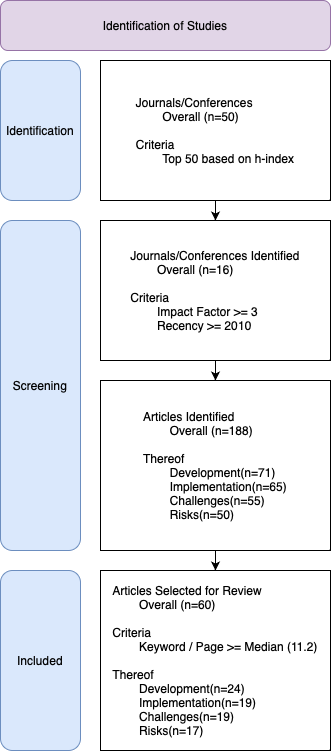
\includegraphics[width=\textwidth,height=\textheight,keepaspectratio]{filtration.png}
    \caption{SLR Process}
\end{figure}
 
The process to find research articles is a simple process in general. Firstly, finding out top 50 journals / conferences using journal quality metrics like H-index/SJR/Impact Score available on Google Scholar / Scimagojr / Resurchify.
These journals were then filtered out journals with papers only on CV / NLP / Robotics, ensuring each journal has relevant research papers on AGI.
Using a sorting and ranking journals based on h-index and recency, select available journals. This narrows it down to 16 journals.
Collect all documents/papers from the last publication year of all the shortlisted journals/conferences, wherever access is possible. Then filtered out irrelevant or duplicate research articles.
From the remaining 188 articles, attempt a keyword search through documents using re and PyPdf2 in Python. Keywords assessed to validate the document were related to AGI were 'general artificial intelligence', 'artificial intelligence', 'artificial general intelligence', 'agi', 'ai', 'artificial', 'intelligence'.
Then, scored each document for the matches found by creating a metric keyword to page ratio and consider only top documents for this score. The remaining 60 documents should be ready for manual review.

To classify documents, check if keywords of each domain are present in the article. Keywords assessed to validate the document were related to development in AGI were 'development', 'design', 'architecture', 'cognitive', 'model', 'cognition', 'paradigm', 'framework', 'brain'. Keywords assessed to validate the document were related to implementation in AGI were 'programming', 'languages', 'hardware', 'neural', 'network', 'evaluation', 'test', 'strength', 'chip', 'algorithm', 'complexity', 'empirical', 'theoretical'. Keywords assessed to validate the document were related to challenges in AGI were 'limitation', 'challenge', 'infrastructure requirement', 'architecture requirement', 'predictive', 'prompt', 'efficiency', 'compute power', 'motivation', 'management', 'difficulty', 'awareness'. Keywords assessed to validate the document were related to risks in AGI were 'consciousness', 'self-aware', 'awareness', 'capabilities' 'safety', 'safe', 'intent', 'rules', 'fears', 'existential', 'fear', 'ethics', 'values'. 
With the documents classified, it was easier to understand and validate our thoughts about the current state of research in each domain.

\section{Results of the Literature Review}

\subsection{Journals / Conferences identified by search terms}

To conduct a survey of high quality documents, several sources of journals and conferences were selected. International Conference on Artificial General Intelligence (ICAGI), International Conference on Learning Representations (ICLR), International Conference on Machine Learning (ICML), Association for the Advancement of Artificial Intelligence (AAAI), Expert Systems with Applications, IEEE Transactions on Neural Networks and Learning Systems, International Joint Conference on Artificial Intelligence (IJCAI).

Initially, top 50 journals and conferences were selected and these were filtered based on median h-index (above 103) and a median impact factor (above 6.46). Finally, there were 16 journals/conferences which were selected.


\subsection{Research Article Frequency per Domain}

    \begin{table}[hbt!]
    	\caption{Articles identified}
    	\centering
        \begin{tabular}{ |p{3cm}||p{3cm}|p{3cm}|p{3cm}|p{3cm}| }
         % \hline
         % \multicolumn{4}{|c|}{Country List} \\
         \hline
         Phase & Development & Implementation & Challenges & Risks \\
         \hline
         Identified Research Articles & 71 & 65 & 55 & 50 \\
         \hline
         Selected Research Articles& 24 & 19 & 19 & 17 \\
         
         \hline
        \end{tabular}
    \label{tab:table3}
    \end{table}

\subsection{Research Article Quality}

Several statistics were collected after selecting the research articles.
Mean and median article length across all articles is respectively 9.3 and 10.
Average and median keyword to page ratio is respectively 11.6 and 8.5.

Across all articles, several metrics were also coined in order to understand prevalence of each topic within the article such as development to page ratio, implementation to page ratio, challenges to page ratio, risks to page ratio. Each topic was understood to be present on a page based on certain keywords selected for each domain.
Average and median development to page ratio is respectively 6.08 and 4.67.
Average and median implementation to page ratio is respectively 3.95 and 2.5.
Average and median challenges to page ratio is respectively 0.26 and 0.57.
Average and median risks to page ratio is respectively 1.23 and 0.68.


\section{Conclusion}
Overall, the research articles that have been identified and selected as part of the SLR process were highly heterogeneous ranging from the computation power of systems to safety of AGI. Most promising approaches were analyzing how humans and AGI can learn from each other to improve these AI systems further. 

In general, there is a still a lot of uncertainty in AGI and it seems like there are a lot of contradictory opinions against newer ideas from fellow researchers. It would be interesting to see how this domain develops as time goes on. In conclusion, there are various starting points for future research in this domain especially in terms of development, implementation, challenges and safety to improve the understanding of AGI to the wider audience and make use of the applications.

\section{Limitations}

Three primary limitations were considered during the process of survey. Search terms were used to filter out research articles as described before. Only top 50 journals and conferences were considered. Articles with high h-index were only used for this survey and time frame of research articles was bound to as early as 2010.

\section{Declaration}

The author(s) declared no potential conflicts of interest with respect to the research, authorship, and/or publication of this article.



\bibliographystyle{unsrtnat}
\bibliography{references}  %%% Uncomment this line and comment out the ``thebibliography'' section below to use the external .bib file (using bibtex) .

\section*{Appendix}

\begin{sidewaystable}
    \caption{Appendix}
    \centering
    \renewcommand{\arraystretch}{3}
    \begin{tabular}{ |p{5cm}|p{10cm}|  }
    \hline
    Author(s) & Objective of Study\\
    \hline
    Mohammadreza Alidoust & In this paper, an index for measuring the versatility of artificial general intelligence (AGI) systems is proposed. The index is called Versatility Index (VI).\\
    
    Roman V. Yampolskiy & In this article, we explore the arguments that advanced AI cannot be completely controlled.\\
    
    Jordi Bieger, Kristinn R. Thórisson, and Deon Garrett & This paper gives a taxonomy of the main methods for raising / educating naturally intelligent systems and provides examples for how these might be applied to artificial systems.\\
    
    Mark R. Waser & This paper talks about the current short-sighted static and reductionist definition of intelligence which focuses on goals must be replaced by a long-term adaptive one focused on learning, growth and self-improvement.\\ 

    Ben Goertzel1, Gino Yu & This paper talks about an Application Programming  Interface for human-level AGI systems is proposed, aimed at bridging the gap between protoAGI R\&D systems and practical AI application development.\\
    
    Roman V. Yampolskiy & In this work, analysis limits on computation which might restrict recursive self-improvement AGI.\\
    
    Jordi Bieger, Kristinn R. Thorisson, and Pei Wang & This paper says that get safe AGI can be created by providing it proper education. \\

    James Babcock, Janos Kramar, and Roman Yampolskiy & In this paper, they survey the AGI containment problem – the question of how to build a container in which tests can be conducted safely and reliably. \\

    Jeremy O. Turner and Steve DiPaola & This paper introduces an interdisciplinary qualitative hermeneutic approach to the engineering and computer science methodological paradigm(s) for assessing a contemplative agent’s cognitive capabilities at a level corresponding to Artificial General Intelligence (AGI). \\

     
    \hline
    \end{tabular}
\end{sidewaystable}

\begin{sidewaystable}
    \caption{Appendix}
    \centering
    \renewcommand{\arraystretch}{3}
    \begin{tabular}{ |p{5cm}|p{10cm}|  }
    \hline
    Author(s) & Objective of Study\\
    \hline
    
    Joscha Bach & In this paper, they describe a framework for an extensible motivational system for cognitive agents, based on research in psychology.\\

    Randal A. Koene & In this paper, they survey that there are serious limitations to the use of cognitive models as inspiration for the components deemed necessary to produce general intelligence.\\

    Diana Deca & The goals of this paper are to review the challenges for gathering and assembling connectome data and to provide directions for overcoming these challenges. \\

    Tarek Richard Besold and Robert Robere & In this paper, they survey artificial intelligence (AI) in its attempt to recreate intelligence and capacities inspired by the human mind is dealing with finite systems \\

    Tarek Richard Besold & In this paper, they argume why HAI should conform to normal scientific standards and methods, using the approach of psychometric artificial intelligence as one of the main foundations of my position. \\

    Hiroshi Yamakawa & In this paper, they desribe how Brain-inspired AGI development, can help reduction of the design space to resemble a biological brain more closely to help develop AGI. \\

    Tom Macpherson, Anne Churchland, Terry Sejnowski, James DiCarlo, Yukiyasu Kamitani, Hidehiko Takahashi, Takatoshi Hikida, & In this paper, they discuss recent advancements in areas in which the relationship between neuroscience and AI has led to major advancements in the field. \\

    Alex Zhavoronkov, Polina Mamoshinaa, Quentin Vanhaelena, Morten Scheiby Knudsene & In this paper, they survey how modern AI is expected to contribute to the credibility and prominence of longevity biotechnology in the healthcare and pharmaceutical industry, and to the convergence of countless areas of research. \\

     
    \hline
    \end{tabular}
\end{sidewaystable}
    

\begin{sidewaystable}
    \caption{Appendix}
    \centering
    \renewcommand{\arraystretch}{3}
    \begin{tabular}{ |p{5cm}|p{10cm}|  }
    \hline
    Author(s) & Objective of Study\\
    \hline
    Nicolas Palanca-Castan, Beatriz Sánchez Tajadura, Rodrigo Cofre & In this paper, they proposes a comparative framework to discuss what we call “purposeful behavior”, a characteristic shared by systems capable of gathering and processing information from their surroundings and modifying their actions in order to fulfill a series of implicit or explicit goals. \\

    Piotr Boltuc & In this paper, they survey definitions of Consciousness of AGI. \\

    Mark R. Waser & In this paper, they describe designing a safe motivational system for intelligent machines \\

    G. Malinetsky, V. Smolin & In this paper, they describe the influence of AGI on real sociality. \\

    Lukas Grundner, Barbara Neuhofer & In this paper, they the bright and dark sides of artificial intelligence. \\

    Zhongzhi Shi, Zeqin Huang & In this paper, they propose a cognitive model of brain-machine integration. \\

    Ross Gruetzemacher, David Paradice & In this paper, they identify an alternative technique called scenario network mapping that is well suited for the difficulties posed in mapping the paths to AGI. \\

    Alexey Potapov, Oleg Scherbakov, Vitaly Bogdanov & In this paper, they analyze elementary school Olympiad math tasks as a possible benchmark for AGI. \\

    Valerio Targon & In this paper, they suggests the existence of a plurality of “general-purpose” AGI paradigms, each specific to a domain of experience. \\

    Vladimir Smolina, Dmitry Zhuravlevb & In this paper, they show AGI as a means of getting "truly" new knowledge using existing experience. \\

    \hline
    \end{tabular}
\end{sidewaystable}

\begin{sidewaystable}
    \caption{Appendix}
    \centering
    \renewcommand{\arraystretch}{3}
    \begin{tabular}{ |p{5cm}|p{10cm}|  }
    \hline
    Author(s) & Objective of Study\\
    \hline
    Albert Efimov & In this paper, they offers comprehensive criticism of the Turing test and develops quality criteria for new artificial general intelligence (AGI) assessment tests. \\

    George Siemensa, Fernando Marmolejo-Ramosa, Florence Gabriel & In this paper, they focus on the relationship between human and artificial cognition and treat these as separate systems, each with distinct strengths and capabilities. \\

    Stephen Casper & In this paper, they present the Achilles Heel hypothesis which states that even a potentially superintelligent system may nonetheless have stable decision-theoretic delusions which cause them to make obviously irrational decisions in adversarial settings. \\

    Pei Wang & In this paper, they survey the evaluation approaches used in AGI research, and argues that the proper way of evaluation is to combine empirical comparison with human intelligence and theoretical analysis of the assumptions and implications of the AGI models. \\

    Brandon Rohrer & In this paper, they propose that an ideal benchmark would possess seven key characteris- tics: fitness, breadth, specificity, low cost, simplicity, range, and task focus. \\ 

    Pei Wang & In this paper, they survey the evaluation approaches used in AGI research, and argues that the proper way of evaluation is to combine empirical comparison with human intelligence and theoretical analysis of the assumptions and implications of the AGI models. \\

    Unmesh Kurup, Nicholas L. Cassimatis & In this paper, they show how the standard DPLL algorithm augmented with diagrammatic reasoning can be used to make SAT more efficient when reasoning about space. \\

    Pedro Demasi & In this paper, they proposes a theoretical framework with formal definitions to distinguish these prob- lems and discuss its use in practical applications and how their properties can be used in order to achieve improvements in the AGI field. \\


    \hline
    \end{tabular}
\end{sidewaystable}

\begin{sidewaystable}
    \caption{Appendix}
    \centering

    \renewcommand{\arraystretch}{3}
    
    \begin{tabular}{ |p{5cm}|p{10cm}|  }
    \hline
    Author(s) & Objective of Study\\
    \hline
    
    Ben Goertzel & In this paper, they propose a methodology is described for estimating these theoretical quantities based on observations of a real biological or artificial system operating in a real environment. \\

    Bill Hibbard & In this paper, they propose using elements of Hutter's agent-environment framework to define a decision support system for simulating, visualizing and analyzing AI designs to understand their consequences. \\

    Sam Freed & In this paper, they discuss how areas in the humanities are introduced as possible inspirations for novel human-like AI. Topics discussed playacting, literature as the field researching both imagination and metaphors, linguistics, music, and hermeneutics. \\

    Nil Geisweiller, Ben Goertzel & In this paper, they discuss why spatiotemporal reasoning is an important skill that an AGI is expected to have, innately or not. \\


    Jose Hernandez-Orallo & In this paper, they address one of the pieces in this puzzle: the definition of a general, unbiased, universal class of environments such that they are appropriate for intelligence tests. \\

    Antonio Chella, Massimo Cossentino & In this paper, they describe a software design of an AGI system based on perception loop. \\

    Antoine van de Ven, Ben A.M. Schouten & In this paper the principle of minimum relative entropy (PMRE) is proposed as a fundamental principle and idea that can be used in the field of AGI. \\

    Seng-Beng Ho & In this paper, they develops just such a general framework, with an approach that emphasizes the fact that the representations involved must be explicitly cognitive and conceptual. \\

    Ray J. Solomonoff & In this paper, they describe ALP, the implementation of it and the features of ALP relevant to its application to AGI. \\

    \hline
    \end{tabular}
\end{sidewaystable}

    

\begin{sidewaystable}
    \caption{Appendix}
    \centering

    \renewcommand{\arraystretch}{3}
    
    \begin{tabular}{ |p{5cm}|p{10cm}|  }
    \hline
    Author(s) & Objective of Study\\
    \hline
    
    Ragnar Fjelland & In this paper, they discuss why general artificial intelligence will not be realized. \\

    Knud Thomsen & In this paper, they propose a novel algorithmic architecture for efficient data processing in living brains and for artificial agents. \\

    Ulf Krumnack, Helmar Gust and Angela Schwering & In this paper, they analyse the meaning (the semantics) of analogical relations that are computed by the analogy engine HDTP (Heuristic-Driven Theory Projection). \\

    Perrin G. Bignoli, Nicholas L. Cassimatis, Arthi Murugesan & In this paper, they introduce a language that encodes the temporal intervals over which relations occur and an integrated system that satisfies constraints formulated in this language. \\

    Laurent Orseau & In this paper, they introduces a system that is able to compress data locally and iteratively, in a relational description language. \\

    Benjamin Johnston & The evaluation of incremental progress towards ‘Strong AI’ or ‘AGI’ remains a challenging open problem. In this paper, we draw inspiration from benchmarks used in artificial commonsense reasoning to propose a new benchmark problem, the Toy Box Problem, that tests the practical real-world intelligence and learning capabilities of an agent. \\
    
    DaeEun Kim & The neuroethology is an interdisciplinary study among artificial intelligence, biology and robotics to understand the animal behavior and its underlying neural mechanism. This paper argues that the neuroethological approach helps understand the general artificial intelligence.\\

    Fernand Gobet, Peter C.R. Lane & This paper argues that the CHREST architecture of cognition can shed important light on developing artificial general intelligence. The key theme is that “cognition is perception.” \\

    \hline
    \end{tabular}
\end{sidewaystable}


    

\begin{sidewaystable}
    \caption{Appendix}
    \centering

    \renewcommand{\arraystretch}{3}
    
    \begin{tabular}{ |p{5cm}|p{10cm}|  }
    \hline
    Author(s) & Objective of Study\\
    \hline
    
    David Kelleya and Mathew Twyman & This paper articulates the methodology and reasoning for how biasing in the Independent Core Observer Model (ICOM) Cognitive Architecture for Artificial General Intelligence (AGI) is done. \\

    Ben Goertzel, Cassio Pennachin, Samir Araujo, Fabricio Silva & In this paper, they describe general intelligence oriented architecture for embodied natural language processing. \\

    David Kelley & This paper shows how the Independent Core Observer Model (ICOM) Cognitive Architecture for Artificial General Intelligence can be applied to intelligence system called mASI. \\

    S. Mason Dambrota & In this paper, they investigate real-time neuromorphic Artificial General Intelligence ecosystems \\

    Eray Ozkural, Cevdet Aykanat & In this paper, they showcase their initial implementation of an Artificial General Intelligence (AGI system) in the O’Caml language with the goal of building Solomonoff’s “Phase 1 machine”.\\

    Jiri Wiedermann & In this paper, they investigate the computational power of artificial general intelligence systems (AGIs). \\

    Daniel Hewlett, Paul Cohen & In this paper, they argue that the ability to find meaningful chunks in sequential input is a core cognitive ability for artificial general intelligence. \\

    G.W. Ng, Y.S. Tan, L.N. Teow, K.H. Ng, K.H. Tan, R.Z. Chan & In this paper, they propose a framework or a cognitive architecture for knowledge exploitation. \\


    \hline
    \end{tabular}
\end{sidewaystable}

    
    
\end{document}
